\documentclass[11pt,a4paper]{article}

% --- Paquetes Esenciales ---
\usepackage[utf8]{inputenc}
\usepackage[spanish,es-nodecimaldot]{babel}
\usepackage[margin=2.2cm]{geometry}
\usepackage{graphicx}
\usepackage{hyperref}
\usepackage{xcolor}
\usepackage{tcolorbox}
\usepackage{listings}
\usepackage{enumitem}
\usepackage{fancyhdr}
\usepackage{titlesec}
\usepackage{booktabs}

% --- Colores Personalizados ---
\definecolor{pokeRed}{RGB}{238, 21, 21}
\definecolor{pokeDark}{RGB}{33, 33, 33}
\definecolor{pokeBlue}{RGB}{59, 76, 202}
\definecolor{pokeGold}{RGB}{255, 203, 5}
\definecolor{codeBg}{RGB}{245, 247, 250}
\definecolor{codeBorder}{RGB}{220, 224, 230}

% --- Configuración de Enlaces e Hipervínculos ---
\hypersetup{
    colorlinks=true,
    linkcolor=pokeRed,
    filecolor=pokeBlue,
    urlcolor=pokeBlue,
    pdftitle={Reporte de Proyecto: Pokédex React API},
    pdfpagemode=FullScreen,
}

% --- Estilos de Cabecera y Pie de Página ---
\pagestyle{fancy}
\fancyhf{}
\fancyhead[L]{\textbf{Pokédex App} | Consumo de API REST}
\fancyhead[R]{\thepage}
\fancyfoot[C]{\footnotesize Desarrollo de Software - Frontend React \& PokeAPI}
\renewcommand{\headrulewidth}{0.8pt}
\renewcommand{\footrulewidth}{0.4pt}

% --- Configuración de Bloques de Código ---
\lstset{
    backgroundcolor=\color{codeBg},
    basicstyle=\ttfamily\footnotesize\color{pokeDark},
    breaklines=true,
    captionpos=b,
    frame=single,
    rulecolor=\color{codeBorder},
    keywordstyle=\color{pokeBlue}\bfseries,
    commentstyle=\color{gray}\itshape,
    stringstyle=\color{pokeRed},
    showstringspaces=false,
    tabsize=2
}

% --- Estilo de Cajas de Información ---
\tcbset{
    colback=white,
    colframe=pokeRed,
    arc=4mm,
    boxrule=1.2pt,
    leftrule=5mm
}

\begin{document}

% --- PORTADA / ENCABEZADO ---
\begin{center}
    {\Huge \textbf{\color{pokeRed} Pokédex React - Consumo de REST API}} \\[0.3cm]
    {\large \textbf{Presentación y Evidencia de Implementación}} \\[0.2cm]
    \rule{\linewidth}{1.2pt} \\[0.3cm]
    \begin{tabular}{ll}
        \textbf{Autor / Estudiante:} & [Tu Nombre Completo] \\
        \textbf{Materia / Curso:} & Desarrollo Web / Frontend \\
        \textbf{Fecha:} & \today \\
        \textbf{Repositorio GitHub:} & \href{https://github.com/yan2005dris-afk/Pokedex.git}{\texttt{https://github.com/yan2005dris-afk/Pokedex.git}} \\
        \textbf{Endpoint Base API:} & \href{https://pokeapi.co/api/v2/pokemon?limit=151}{\texttt{https://pokeapi.co/api/v2/pokemon?limit=151}} \\
    \end{tabular}
\end{center}

\vspace{0.3cm}

% --- SECCIÓN 1: OBJETIVOS Y DESCRIPCIÓN ---
\section{Descripción del Software y Objetivos}

El presente proyecto consiste en el desarrollo de una aplicación web interactiva desarrollada con el framework \textbf{React 19}, \textbf{TypeScript} y \textbf{Tailwind CSS 4}, empaquetada mediante \textbf{Vite}. La aplicación consume en tiempo real los datos proporcionados por la API pública de Pokémon (\textit{PokéAPI}), consultando y procesando la información de los primeros \textbf{151 Pokémon} (Generación I).

\subsection*{Funcionalidades Clave Implementadas}
\begin{itemize}[leftmargin=*]
    \item \textbf{Carga y Paginación/Batching Asíncrono:} Consumo de los 151 Pokémon iniciales utilizando \texttt{fetch} con procesamiento concurrente por bloques y almacenamiento en caché en memoria para evitar saturación de red.
    \item \textbf{Búsqueda y Filtrado Dinámico:} Búsqueda en tiempo real por nombre/ID y filtrado por tipos elementales (Fuego, Agua, Planta, Eléctrico, etc.).
    \item \textbf{Vista de Detalle (Modal):} Consulta detallada con estadísticas base (HP, Ataque, Defensa, Velocidad, etc.), tipos, peso, altura y habilidades.
    \item \textbf{Constructor de Equipo (Team Builder):} Permite armar un equipo de hasta 6 Pokémon con persistencia reactiva en el estado de la aplicación.
    \item \textbf{Diseño Responsivo:} Adaptado a dispositivos móviles, tablets y monitores de escritorio.
\end{itemize}

% --- SECCIÓN 2: ARQUITECTURA Y TECNOLOGÍAS ---
\section{Stack Tecnológico y Arquitectura}

\begin{table}[h!]
\centering
\begin{tabular}{@{}lll@{}}
\toprule
\textbf{Capa / Rol} & \textbf{Tecnología} & \textbf{Descripción} \\ \midrule
Frontend Framework & React 19 + TypeScript & Componentes funcionales y tipado estricto \\
Build Tool & Vite 8 & Servidor de desarrollo ultrarrápido y empaquetado \\
Estilos / UI & Tailwind CSS 4 & Diseño atómico utilitario y responsivo \\
Iconografía & Lucide React & Íconos vectoriales modernos y optimizados \\
Fuente de Datos & PokeAPI v2 & API REST pública (\texttt{/pokemon?limit=151}) \\
Control de Versiones & Git \& GitHub & Gestión de versiones con Conventional Commits \\ \bottomrule
\end{tabular}
\caption{Stack tecnológico del proyecto}
\end{table}

% --- SECCIÓN 3: CONSUMO DE LA API ---
\section{Consumo de la API REST}

Para garantizar un rendimiento óptimo y no bloquear la interfaz, el servicio de conexión implementa peticiones concurrentes y caché:

\begin{lstlisting}[language=Java, caption={Servicio de consumo en TypeScript (\texttt{src/services/pokemonService.ts})}]
const API_BASE_URL = 'https://pokeapi.co/api/v2';

export async function fetchPokemonList(limit: number = 151): Promise<PokemonListResponse> {
  const response = await fetch(`${API_BASE_URL}/pokemon?limit=${limit}`);
  if (!response.ok) {
    throw new Error(`Error ${response.status}: Failed to fetch Pokemon list`);
  }
  return response.json();
}
\end{lstlisting}

% --- SECCIÓN 4: GUÍA PARA LEVANTAR EL PROYECTO ---
\section{Instrucciones para Despliegue en Entorno Local}

Para clonar, instalar dependencias y levantar el servidor local de desarrollo, ejecute los siguientes comandos en su terminal:

\begin{tcolorbox}[title=\textbf{Comandos de Instalación y Ejecución}]
\begin{lstlisting}[language=bash]
# 1. Clonar el repositorio
git clone https://github.com/yan2005dris-afk/Pokedex.git
cd Pokedex

# 2. Instalar dependencias (con npm o pnpm)
pnpm install
# o: npm install

# 3. Iniciar el servidor de desarrollo local
pnpm run dev
# o: npm run dev
\end{lstlisting}
\end{tcolorbox}

\noindent El proyecto quedará accesible localmente en la URL por defecto: \href{http://localhost:5173}{\texttt{http://localhost:5173}}.

\newpage

% --- SECCIÓN 5: CAPTURAS DE PANTALLA Y EVIDENCIA ---
\section{Capturas de Pantalla y Evidencia de Funcionamiento}

\noindent \textit{Nota: Inserte las capturas de pantalla de la aplicación ejecutándose en su entorno local en los siguientes recuadros.}

\vspace{0.3cm}

\subsection{1. Vista Principal del Catálogo (151 Pokémon y Filtros)}
\begin{figure}[h!]
    \centering
    % Descomente y reemplace con la ruta a su imagen:
    % 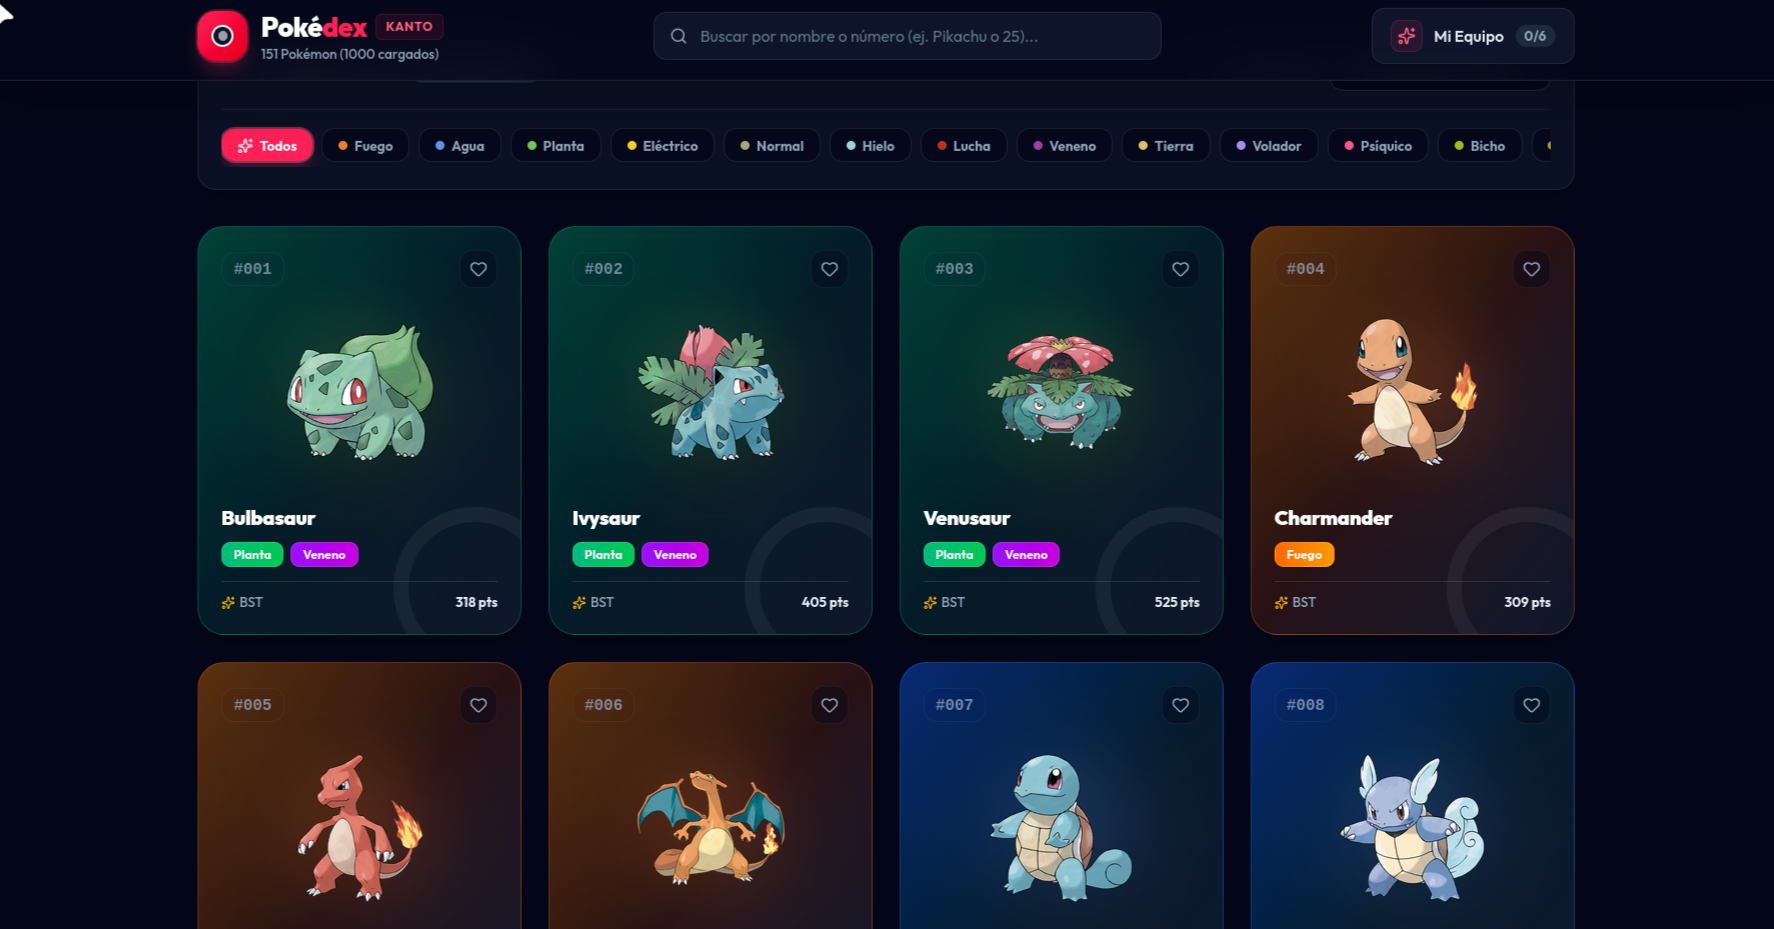
\includegraphics[width=0.9\textwidth]{capturas/01_catalogo.png}
    \begin{tcolorbox}[height=6cm, halign=center, valign=center, colback=gray!10, colframe=gray!50]
        \textbf{[ Captura de Pantalla 1: Vista Principal / Listado de Pokémon ]} \\
        \small Inserte aquí la captura del home mostrando el grid de Pokémon, barra de búsqueda y filtros.
    \end{tcolorbox}
    \caption{Interfaz principal con el catálogo cargado desde PokeAPI.}
\end{figure}

\subsection{2. Búsqueda y Filtrado por Tipo}
\begin{figure}[h!]
    \centering
    % 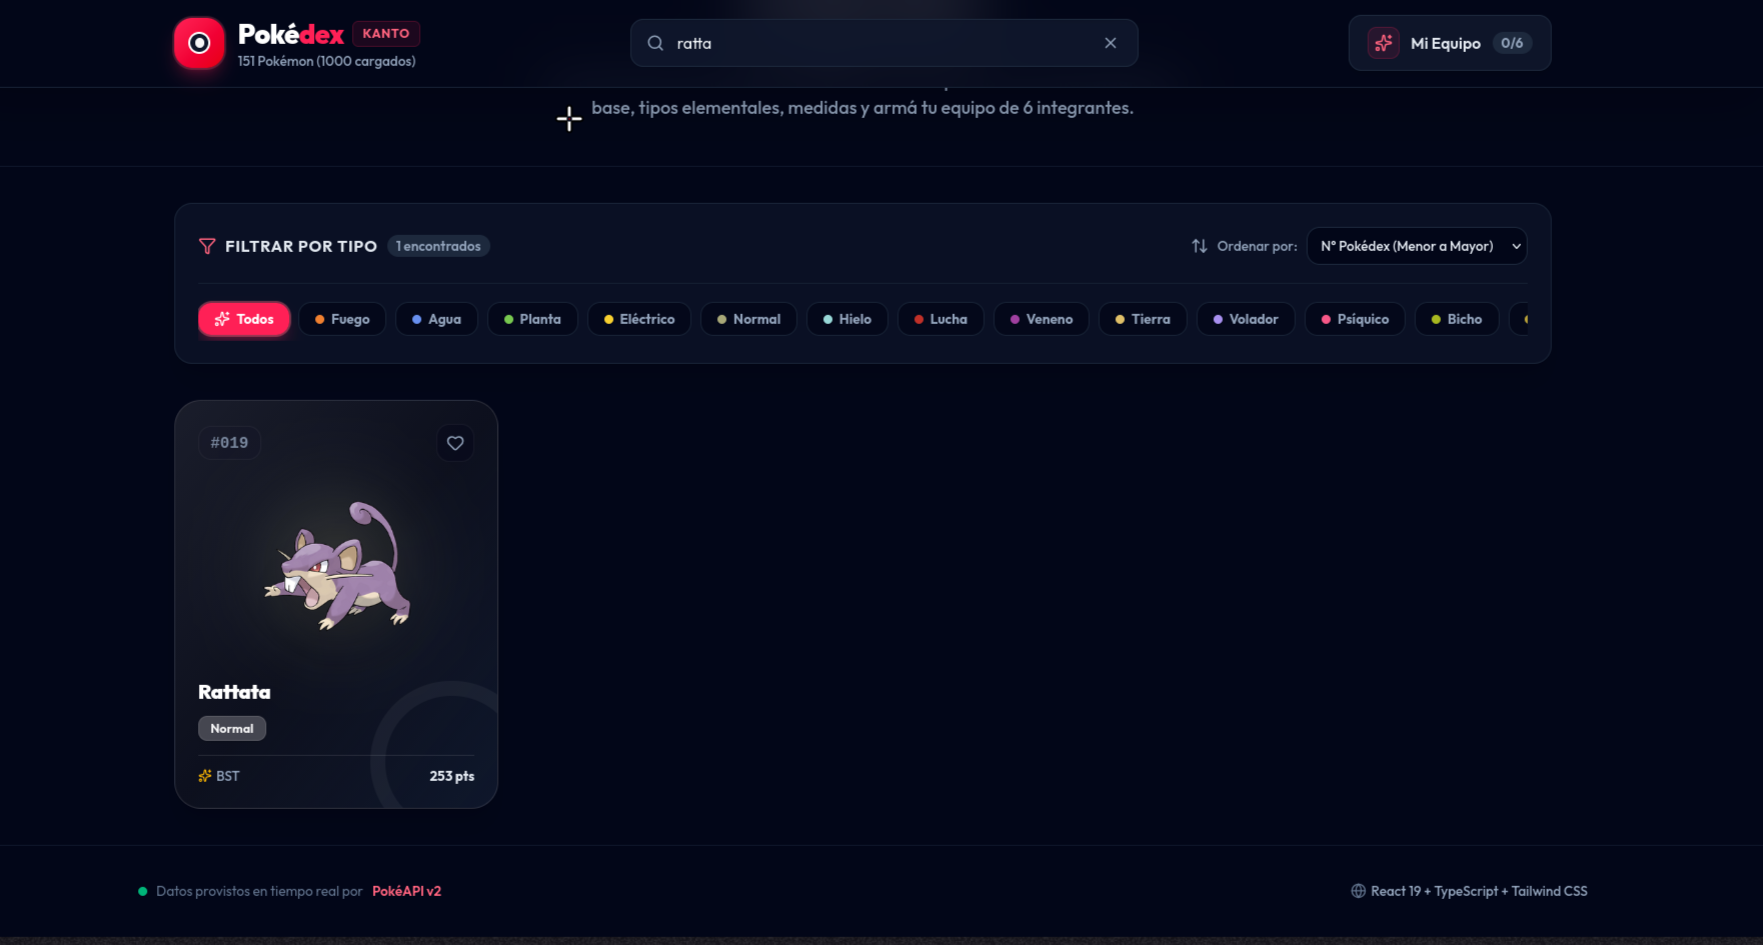
\includegraphics[width=0.9\textwidth]{capturas/02_filtros.png}
    \begin{tcolorbox}[height=5.5cm, halign=center, valign=center, colback=gray!10, colframe=gray!50]
        \textbf{[ Captura de Pantalla 2: Filtrado por Tipo o Búsqueda ]} \\
        \small Inserte aquí la captura mostrando los resultados filtrados por un tipo específico (ej. Fuego / Agua) o búsqueda por texto.
    \end{tcolorbox}
    \caption{Resultado del filtrado reactivo en tiempo real.}
\end{figure}

\newpage

\subsection{3. Vista Modal de Detalle de Pokémon}
\begin{figure}[h!]
    \centering
    % 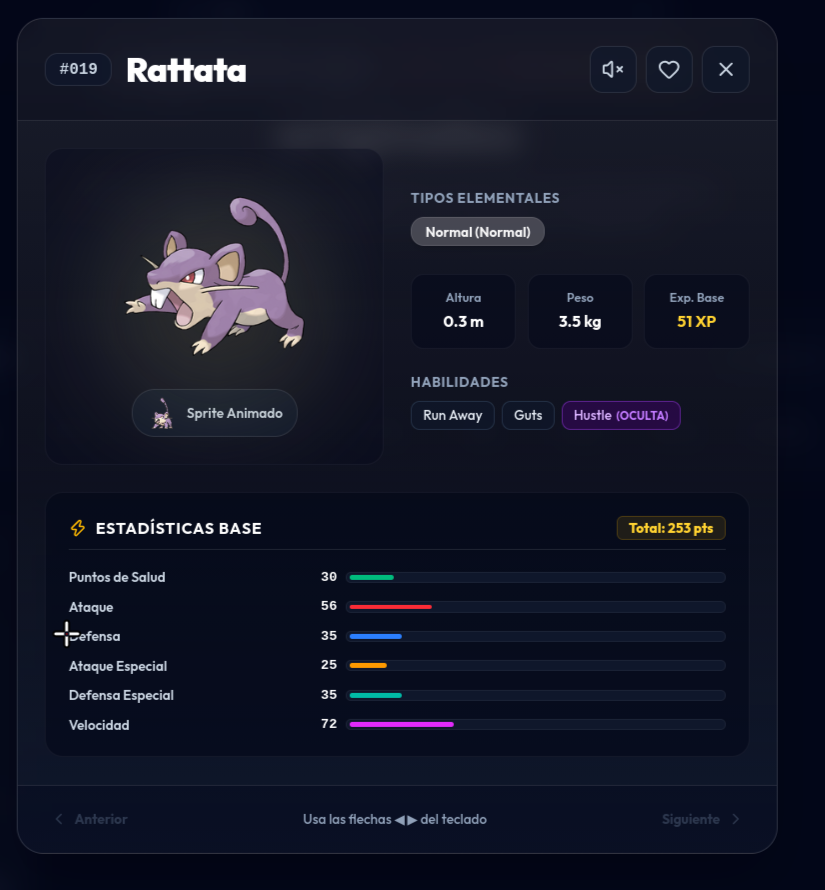
\includegraphics[width=0.85\textwidth]{capturas/03_modal_detalle.png}
    \begin{tcolorbox}[height=6.5cm, halign=center, valign=center, colback=gray!10, colframe=gray!50]
        \textbf{[ Captura de Pantalla 3: Modal de Estadísticas Detalladas ]} \\
        \small Inserte aquí la captura del modal abierto al hacer click sobre una tarjeta, mostrando stats, peso, altura y habilidades.
    \end{tcolorbox}
    \caption{Modal interactivo con datos detallados del Pokémon seleccionado.}
\end{figure}

\subsection{4. Panel del Equipo Pokémon (Team Drawer)}
\begin{figure}[h!]
    \centering
    % 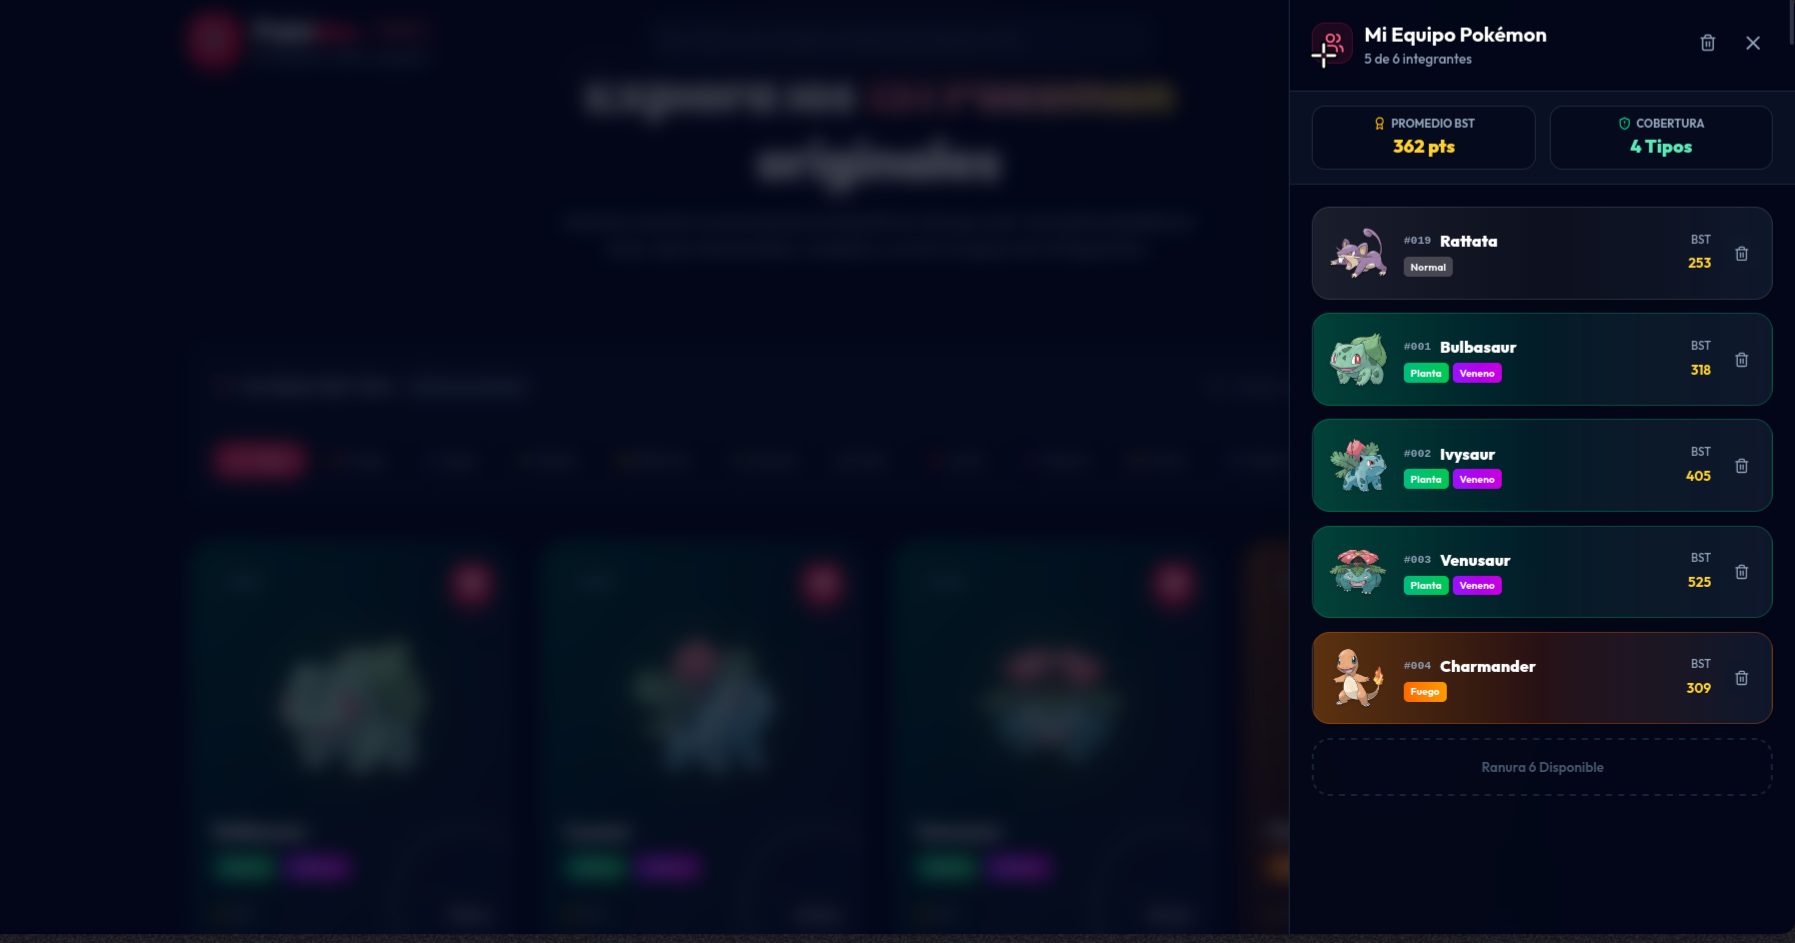
\includegraphics[width=0.85\textwidth]{capturas/04_team_drawer.png}
    \begin{tcolorbox}[height=6cm, halign=center, valign=center, colback=gray!10, colframe=gray!50]
        \textbf{[ Captura de Pantalla 4: Gestión de Equipo (Team Drawer) ]} \\
        \small Inserte aquí la captura del panel lateral con los Pokémon seleccionados en el equipo de 6.
    \end{tcolorbox}
    \caption{Módulo de gestión y visualización del equipo Pokémon.}
\end{figure}

% --- SECCIÓN 6: CONCLUSIONES ---
\section{Conclusiones}
\begin{itemize}[leftmargin=*]
    \item La separación en capas (servicios, componentes UI, tipos TypeScript) permitió un código modular, mantenible y escalable.
    \item El manejo asíncrono con control de concurrencia y caché garantiza una experiencia fluida sin cuellos de botella ni bloqueos de red al consultar la API externa.
\end{itemize}

\end{document}
